% 2017_shanghai_spring_q17_fig1: cuboid ABCD-A1B1C1D1 with triangle A1-B-C.
% Bottom ABCD, top A1B1C1D1; hidden D edges dashed; A1-B solid, A1-D/A1-C dashed.
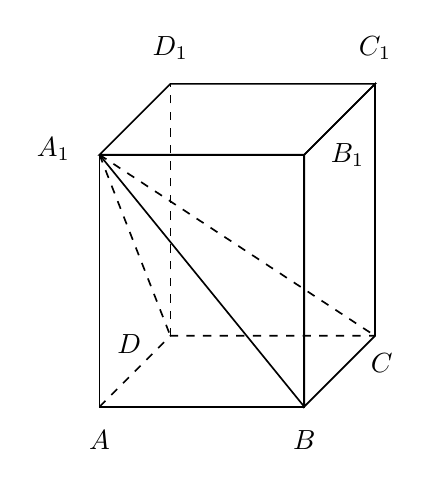
\begin{tikzpicture}[x=1cm,y=1cm,font=\normalsize,line width=.6pt]
\coordinate (A) at (0,0);
\coordinate (B) at (2.6,0);
\coordinate (C) at (3.5,0.9);
\coordinate (D) at (0.9,0.9);
\coordinate (A1) at (0,3.2);
\coordinate (B1) at (2.6,3.2);
\coordinate (C1) at (3.5,4.1);
\coordinate (D1) at (0.9,4.1);
% cuboid outline
\draw[solid,line width=.6pt] (A)--(B)--(B1)--(A1)--cycle;
\draw[solid,line width=.6pt] (B)--(C)--(C1)--(B1)--cycle;
\draw[solid,line width=.6pt] (A1)--(B1)--(C1)--(D1)--cycle;
\draw[solid,line width=.6pt] (A)--(A1);
\draw[solid,line width=.6pt] (C)--(C1);
\draw[dashed,line width=.6pt] (A)--(D)--(C);
\draw[dashed,line width=.6pt] (D)--(D1);
% triangle A1-B-C
\draw[solid,line width=.6pt] (A1)--(B);
\draw[dashed,line width=.6pt] (A1)--(D);
\draw[dashed,line width=.6pt] (A1)--(C);
\node[anchor=north,yshift=-5pt] at (A) {$A$};
\node[anchor=north,yshift=-5pt] at (B) {$B$};
\node[anchor=east,xshift=10pt,yshift=-10pt] at (C) {$C$};
\node[anchor=north east,xshift=-7pt,yshift=4pt] at (D) {$D$};
\node[anchor=east,xshift=-7pt,yshift=2pt] at (A1) {$A_{1}$};
\node[anchor=west,xshift=6pt] at (B1) {$B_{1}$};
\node[anchor=south,yshift=5pt] at (C1) {$C_{1}$};
\node[anchor=south,yshift=5pt] at (D1) {$D_{1}$};
\end{tikzpicture}
